\documentclass{standalone}
\usepackage{tikz}
\usetikzlibrary{patterns, positioning}


\begin{document}
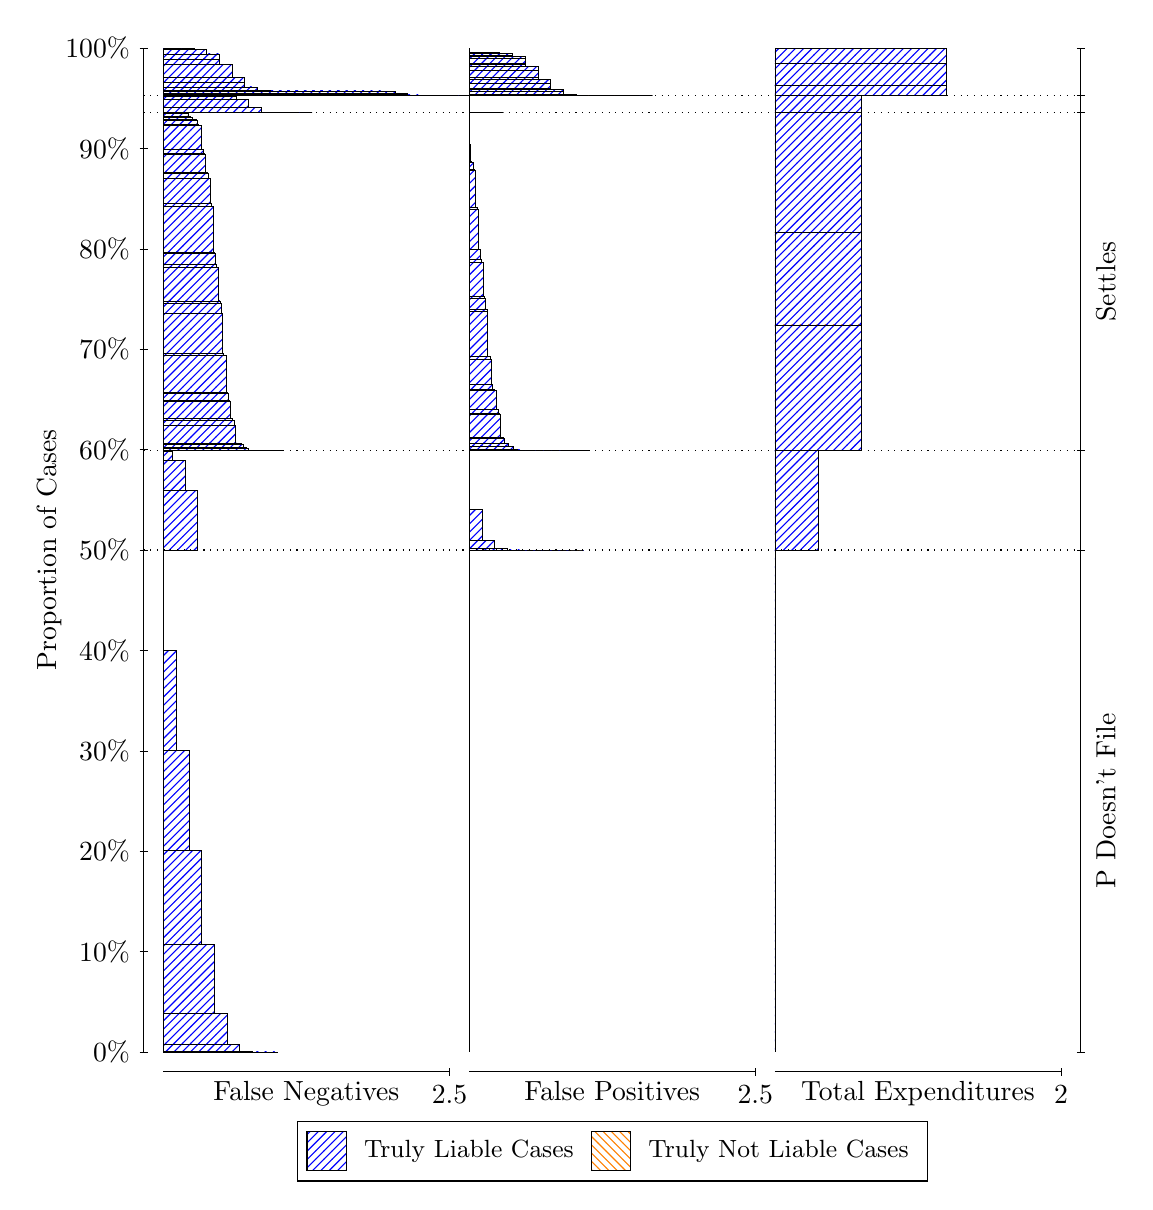
\begin{tikzpicture}
\draw[black, very thin] (1.5,1.75) -- (1.5,14.5);
\node[rotate=90, text=black, anchor=center] at (0.3, 8.125) {Proportion of Cases};
\draw[black, very thin] (1.45,1.75) -- (1.55,1.75);
\node[text=black, anchor=east] at (1.45, 1.75) {0\%};
\draw[black, very thin] (1.45,3.025) -- (1.55,3.025);
\node[text=black, anchor=east] at (1.45, 3.025) {10\%};
\draw[black, very thin] (1.45,4.3) -- (1.55,4.3);
\node[text=black, anchor=east] at (1.45, 4.3) {20\%};
\draw[black, very thin] (1.45,5.575) -- (1.55,5.575);
\node[text=black, anchor=east] at (1.45, 5.575) {30\%};
\draw[black, very thin] (1.45,6.85) -- (1.55,6.85);
\node[text=black, anchor=east] at (1.45, 6.85) {40\%};
\draw[black, very thin] (1.45,8.125) -- (1.55,8.125);
\node[text=black, anchor=east] at (1.45, 8.125) {50\%};
\draw[black, very thin] (1.45,9.4) -- (1.55,9.4);
\node[text=black, anchor=east] at (1.45, 9.4) {60\%};
\draw[black, very thin] (1.45,10.675) -- (1.55,10.675);
\node[text=black, anchor=east] at (1.45, 10.675) {70\%};
\draw[black, very thin] (1.45,11.95) -- (1.55,11.95);
\node[text=black, anchor=east] at (1.45, 11.95) {80\%};
\draw[black, very thin] (1.45,13.225) -- (1.55,13.225);
\node[text=black, anchor=east] at (1.45, 13.225) {90\%};
\draw[black, very thin] (1.45,14.5) -- (1.55,14.5);
\node[text=black, anchor=east] at (1.45, 14.5) {100\%};

\draw[black, very thin] (13.4,1.75) -- (13.4,14.5);
\draw[black, very thin] (13.35,1.75) -- (13.45,1.75);
\node[anchor=west] at (13.35, 1.75) {};
\draw[black, very thin] (13.35,8.125) -- (13.45,8.125);
\node[anchor=west] at (13.35, 8.125) {};
\draw[black, very thin] (13.35,9.3926) -- (13.45,9.3926);
\node[anchor=west] at (13.35, 9.3926) {};
\draw[black, very thin] (13.35,13.68) -- (13.45,13.68);
\node[anchor=west] at (13.35, 13.68) {};
\draw[black, very thin] (13.35,13.898) -- (13.45,13.898);
\node[anchor=west] at (13.35, 13.898) {};
\draw[black, very thin] (13.35,14.5) -- (13.45,14.5);
\node[anchor=west] at (13.35, 14.5) {};

\draw[black, very thin, pattern color=blue, pattern=north east lines] (1.75,1.75) rectangle (3.2033,1.75);
\draw[black, very thin, pattern color=blue, pattern=north east lines] (1.75,1.75) rectangle (3.0419,1.7503);
\draw[black, very thin, pattern color=blue, pattern=north east lines] (1.75,1.7503) rectangle (2.8804,1.7583);
\draw[black, very thin, pattern color=blue, pattern=north east lines] (1.75,1.7583) rectangle (2.7189,1.8435);
\draw[black, very thin, pattern color=blue, pattern=north east lines] (1.75,1.8435) rectangle (2.5574,2.2369);
\draw[black, very thin, pattern color=blue, pattern=north east lines] (1.75,2.2369) rectangle (2.3959,3.1185);
\draw[black, very thin, pattern color=blue, pattern=north east lines] (1.75,3.1185) rectangle (2.2344,4.3083);
\draw[black, very thin, pattern color=blue, pattern=north east lines] (1.75,4.3083) rectangle (2.073,5.5753);
\draw[black, very thin, pattern color=blue, pattern=north east lines] (1.75,5.5753) rectangle (1.9115,6.85);
\draw[black, very thin, pattern color=orange, pattern=north west lines] (1.75,6.85) rectangle (1.75,6.85);
\draw[black, very thin, pattern color=blue, pattern=north east lines] (1.75,6.85) rectangle (1.75,8.125);
\draw[black, very thin, pattern color=blue, pattern=north east lines] (1.75,8.125) rectangle (2.186,8.8794);
\draw[black, very thin, pattern color=blue, pattern=north east lines] (1.75,8.8794) rectangle (2.0245,9.2662);
\draw[black, very thin, pattern color=blue, pattern=north east lines] (1.75,9.2662) rectangle (1.863,9.3769);
\draw[black, very thin, pattern color=orange, pattern=north west lines] (1.75,9.3769) rectangle (1.75,9.3769);
\draw[black, very thin, pattern color=blue, pattern=north east lines] (1.75,9.3769) rectangle (1.75,9.3926);
\draw[black, very thin, pattern color=blue, pattern=north east lines] (1.75,9.3926) rectangle (3.276,9.3926);
\draw[black, very thin, pattern color=blue, pattern=north east lines] (1.75,9.3926) rectangle (3.2033,9.3926);
\draw[black, very thin, pattern color=blue, pattern=north east lines] (1.75,9.3926) rectangle (3.1307,9.3926);
\draw[black, very thin, pattern color=blue, pattern=north east lines] (1.75,9.3926) rectangle (3.1145,9.3926);
\draw[black, very thin, pattern color=blue, pattern=north east lines] (1.75,9.3926) rectangle (3.058,9.3926);
\draw[black, very thin, pattern color=blue, pattern=north east lines] (1.75,9.3926) rectangle (3.0419,9.3926);
\draw[black, very thin, pattern color=blue, pattern=north east lines] (1.75,9.3926) rectangle (2.9853,9.3935);
\draw[black, very thin, pattern color=blue, pattern=north east lines] (1.75,9.3935) rectangle (2.9692,9.3937);
\draw[black, very thin, pattern color=blue, pattern=north east lines] (1.75,9.3937) rectangle (2.953,9.3937);
\draw[black, very thin, pattern color=blue, pattern=north east lines] (1.75,9.3937) rectangle (2.9127,9.3938);
\draw[black, very thin, pattern color=blue, pattern=north east lines] (1.75,9.3938) rectangle (2.8965,9.394);
\draw[black, very thin, pattern color=blue, pattern=north east lines] (1.75,9.394) rectangle (2.8804,9.3941);
\draw[black, very thin, pattern color=blue, pattern=north east lines] (1.75,9.3941) rectangle (2.84,9.3942);
\draw[black, very thin, pattern color=blue, pattern=north east lines] (1.75,9.3942) rectangle (2.8239,9.4188);
\draw[black, very thin, pattern color=blue, pattern=north east lines] (1.75,9.4188) rectangle (2.8077,9.4268);
\draw[black, very thin, pattern color=blue, pattern=north east lines] (1.75,9.4268) rectangle (2.7916,9.4295);
\draw[black, very thin, pattern color=blue, pattern=north east lines] (1.75,9.4295) rectangle (2.7673,9.4691);
\draw[black, very thin, pattern color=blue, pattern=north east lines] (1.75,9.4691) rectangle (2.7512,9.4708);
\draw[black, very thin, pattern color=blue, pattern=north east lines] (1.75,9.4708) rectangle (2.735,9.4812);
\draw[black, very thin, pattern color=blue, pattern=north east lines] (1.75,9.4812) rectangle (2.7189,9.4839);
\draw[black, very thin, pattern color=blue, pattern=north east lines] (1.75,9.4839) rectangle (2.6785,9.4861);
\draw[black, very thin, pattern color=blue, pattern=north east lines] (1.75,9.4861) rectangle (2.6624,9.7044);
\draw[black, very thin, pattern color=blue, pattern=north east lines] (1.75,9.7044) rectangle (2.6462,9.7732);
\draw[black, very thin, pattern color=blue, pattern=north east lines] (1.75,9.7732) rectangle (2.6301,9.7945);
\draw[black, very thin, pattern color=blue, pattern=north east lines] (1.75,9.7945) rectangle (2.6059,10.01);
\draw[black, very thin, pattern color=blue, pattern=north east lines] (1.75,10.01) rectangle (2.5897,10.026);
\draw[black, very thin, pattern color=blue, pattern=north east lines] (1.75,10.026) rectangle (2.5736,10.111);
\draw[black, very thin, pattern color=blue, pattern=north east lines] (1.75,10.111) rectangle (2.5574,10.128);
\draw[black, very thin, pattern color=blue, pattern=north east lines] (1.75,10.128) rectangle (2.5493,10.598);
\draw[black, very thin, pattern color=blue, pattern=north east lines] (1.75,10.598) rectangle (2.517,10.618);
\draw[black, very thin, pattern color=blue, pattern=north east lines] (1.75,10.618) rectangle (2.5009,11.128);
\draw[black, very thin, pattern color=blue, pattern=north east lines] (1.75,11.128) rectangle (2.4847,11.259);
\draw[black, very thin, pattern color=blue, pattern=north east lines] (1.75,11.259) rectangle (2.4686,11.29);
\draw[black, very thin, pattern color=blue, pattern=north east lines] (1.75,11.29) rectangle (2.4444,11.721);
\draw[black, very thin, pattern color=blue, pattern=north east lines] (1.75,11.721) rectangle (2.4282,11.751);
\draw[black, very thin, pattern color=blue, pattern=north east lines] (1.75,11.751) rectangle (2.4121,11.893);
\draw[black, very thin, pattern color=blue, pattern=north east lines] (1.75,11.893) rectangle (2.3959,11.91);
\draw[black, very thin, pattern color=blue, pattern=north east lines] (1.75,11.91) rectangle (2.3879,12.487);
\draw[black, very thin, pattern color=blue, pattern=north east lines] (1.75,12.487) rectangle (2.3556,12.527);
\draw[black, very thin, pattern color=blue, pattern=north east lines] (1.75,12.527) rectangle (2.3394,12.849);
\draw[black, very thin, pattern color=blue, pattern=north east lines] (1.75,12.849) rectangle (2.3233,12.909);
\draw[black, very thin, pattern color=blue, pattern=north east lines] (1.75,12.909) rectangle (2.3071,12.918);
\draw[black, very thin, pattern color=blue, pattern=north east lines] (1.75,12.918) rectangle (2.2829,13.155);
\draw[black, very thin, pattern color=blue, pattern=north east lines] (1.75,13.155) rectangle (2.2667,13.166);
\draw[black, very thin, pattern color=blue, pattern=north east lines] (1.75,13.166) rectangle (2.2506,13.215);
\draw[black, very thin, pattern color=blue, pattern=north east lines] (1.75,13.215) rectangle (2.2344,13.218);
\draw[black, very thin, pattern color=blue, pattern=north east lines] (1.75,13.218) rectangle (2.2264,13.515);
\draw[black, very thin, pattern color=blue, pattern=north east lines] (1.75,13.515) rectangle (2.1941,13.529);
\draw[black, very thin, pattern color=blue, pattern=north east lines] (1.75,13.529) rectangle (2.1779,13.586);
\draw[black, very thin, pattern color=blue, pattern=north east lines] (1.75,13.586) rectangle (2.1618,13.592);
\draw[black, very thin, pattern color=blue, pattern=north east lines] (1.75,13.592) rectangle (2.1456,13.593);
\draw[black, very thin, pattern color=blue, pattern=north east lines] (1.75,13.593) rectangle (2.1214,13.624);
\draw[black, very thin, pattern color=blue, pattern=north east lines] (1.75,13.624) rectangle (2.1053,13.625);
\draw[black, very thin, pattern color=blue, pattern=north east lines] (1.75,13.625) rectangle (2.0891,13.629);
\draw[black, very thin, pattern color=blue, pattern=north east lines] (1.75,13.629) rectangle (2.073,13.629);
\draw[black, very thin, pattern color=blue, pattern=north east lines] (1.75,13.629) rectangle (2.0649,13.673);
\draw[black, very thin, pattern color=blue, pattern=north east lines] (1.75,13.673) rectangle (2.0326,13.674);
\draw[black, very thin, pattern color=blue, pattern=north east lines] (1.75,13.674) rectangle (2.0164,13.677);
\draw[black, very thin, pattern color=blue, pattern=north east lines] (1.75,13.677) rectangle (2.0003,13.677);
\draw[black, very thin, pattern color=blue, pattern=north east lines] (1.75,13.677) rectangle (1.9841,13.677);
\draw[black, very thin, pattern color=blue, pattern=north east lines] (1.75,13.677) rectangle (1.9599,13.678);
\draw[black, very thin, pattern color=blue, pattern=north east lines] (1.75,13.678) rectangle (1.9438,13.678);
\draw[black, very thin, pattern color=blue, pattern=north east lines] (1.75,13.678) rectangle (1.9276,13.678);
\draw[black, very thin, pattern color=blue, pattern=north east lines] (1.75,13.678) rectangle (1.9115,13.678);
\draw[black, very thin, pattern color=blue, pattern=north east lines] (1.75,13.678) rectangle (1.9034,13.68);
\draw[black, very thin, pattern color=blue, pattern=north east lines] (1.75,13.68) rectangle (1.8711,13.68);
\draw[black, very thin, pattern color=blue, pattern=north east lines] (1.75,13.68) rectangle (1.855,13.68);
\draw[black, very thin, pattern color=blue, pattern=north east lines] (1.75,13.68) rectangle (1.8388,13.68);
\draw[black, very thin, pattern color=blue, pattern=north east lines] (1.75,13.68) rectangle (1.8227,13.68);
\draw[black, very thin, pattern color=blue, pattern=north east lines] (1.75,13.68) rectangle (1.7984,13.68);
\draw[black, very thin, pattern color=blue, pattern=north east lines] (1.75,13.68) rectangle (1.7823,13.68);
\draw[black, very thin, pattern color=blue, pattern=north east lines] (1.75,13.68) rectangle (1.7661,13.68);
\draw[black, very thin, pattern color=orange, pattern=north west lines] (1.75,13.68) rectangle (1.75,13.68);
\draw[black, very thin, pattern color=blue, pattern=north east lines] (1.75,13.68) rectangle (1.75,13.68);
\draw[black, very thin, pattern color=blue, pattern=north east lines] (1.75,13.68) rectangle (3.6393,13.68);
\draw[black, very thin, pattern color=blue, pattern=north east lines] (1.75,13.68) rectangle (3.4779,13.68);
\draw[black, very thin, pattern color=blue, pattern=north east lines] (1.75,13.68) rectangle (3.3164,13.68);
\draw[black, very thin, pattern color=blue, pattern=north east lines] (1.75,13.68) rectangle (3.1549,13.687);
\draw[black, very thin, pattern color=blue, pattern=north east lines] (1.75,13.687) rectangle (2.9934,13.746);
\draw[black, very thin, pattern color=blue, pattern=north east lines] (1.75,13.746) rectangle (2.8319,13.848);
\draw[black, very thin, pattern color=blue, pattern=north east lines] (1.75,13.848) rectangle (2.6704,13.892);
\draw[black, very thin, pattern color=blue, pattern=north east lines] (1.75,13.892) rectangle (2.509,13.898);
\draw[black, very thin, pattern color=blue, pattern=north east lines] (1.75,13.898) rectangle (2.3475,13.898);
\draw[black, very thin, pattern color=blue, pattern=north east lines] (1.75,13.898) rectangle (2.186,13.898);
\draw[black, very thin, pattern color=orange, pattern=north west lines] (1.75,13.898) rectangle (1.75,13.898);
\draw[black, very thin, pattern color=blue, pattern=north east lines] (1.75,13.898) rectangle (5.8193,13.898);
\draw[black, very thin, pattern color=blue, pattern=north east lines] (1.75,13.898) rectangle (5.6579,13.898);
\draw[black, very thin, pattern color=blue, pattern=north east lines] (1.75,13.898) rectangle (5.4964,13.898);
\draw[black, very thin, pattern color=blue, pattern=north east lines] (1.75,13.898) rectangle (5.3349,13.898);
\draw[black, very thin, pattern color=blue, pattern=north east lines] (1.75,13.898) rectangle (5.3349,13.898);
\draw[black, very thin, pattern color=blue, pattern=north east lines] (1.75,13.898) rectangle (5.1734,13.899);
\draw[black, very thin, pattern color=blue, pattern=north east lines] (1.75,13.899) rectangle (5.0119,13.903);
\draw[black, very thin, pattern color=blue, pattern=north east lines] (1.75,13.903) rectangle (5.0119,13.904);
\draw[black, very thin, pattern color=blue, pattern=north east lines] (1.75,13.904) rectangle (4.8504,13.915);
\draw[black, very thin, pattern color=blue, pattern=north east lines] (1.75,13.915) rectangle (4.8504,13.922);
\draw[black, very thin, pattern color=blue, pattern=north east lines] (1.75,13.922) rectangle (4.689,13.947);
\draw[black, very thin, pattern color=blue, pattern=north east lines] (1.75,13.947) rectangle (4.5275,13.954);
\draw[black, very thin, pattern color=blue, pattern=north east lines] (1.75,13.954) rectangle (4.5275,13.956);
\draw[black, very thin, pattern color=blue, pattern=north east lines] (1.75,13.956) rectangle (4.366,13.956);
\draw[black, very thin, pattern color=blue, pattern=north east lines] (1.75,13.956) rectangle (4.2045,13.956);
\draw[black, very thin, pattern color=blue, pattern=north east lines] (1.75,13.956) rectangle (4.043,13.956);
\draw[black, very thin, pattern color=blue, pattern=north east lines] (1.75,13.956) rectangle (4.043,13.956);
\draw[black, very thin, pattern color=blue, pattern=north east lines] (1.75,13.956) rectangle (3.8816,13.956);
\draw[black, very thin, pattern color=blue, pattern=north east lines] (1.75,13.956) rectangle (3.7524,13.956);
\draw[black, very thin, pattern color=blue, pattern=north east lines] (1.75,13.956) rectangle (3.7201,13.956);
\draw[black, very thin, pattern color=blue, pattern=north east lines] (1.75,13.956) rectangle (3.5909,13.956);
\draw[black, very thin, pattern color=blue, pattern=north east lines] (1.75,13.956) rectangle (3.4294,13.956);
\draw[black, very thin, pattern color=blue, pattern=north east lines] (1.75,13.956) rectangle (3.2679,13.956);
\draw[black, very thin, pattern color=blue, pattern=north east lines] (1.75,13.956) rectangle (3.2679,13.956);
\draw[black, very thin, pattern color=blue, pattern=north east lines] (1.75,13.956) rectangle (3.1064,13.959);
\draw[black, very thin, pattern color=blue, pattern=north east lines] (1.75,13.959) rectangle (3.1064,13.962);
\draw[black, very thin, pattern color=blue, pattern=north east lines] (1.75,13.962) rectangle (2.945,14.007);
\draw[black, very thin, pattern color=blue, pattern=north east lines] (1.75,14.007) rectangle (2.7835,14.069);
\draw[black, very thin, pattern color=blue, pattern=north east lines] (1.75,14.069) rectangle (2.7835,14.131);
\draw[black, very thin, pattern color=blue, pattern=north east lines] (1.75,14.131) rectangle (2.622,14.295);
\draw[black, very thin, pattern color=blue, pattern=north east lines] (1.75,14.295) rectangle (2.4605,14.358);
\draw[black, very thin, pattern color=blue, pattern=north east lines] (1.75,14.358) rectangle (2.4605,14.361);
\draw[black, very thin, pattern color=blue, pattern=north east lines] (1.75,14.361) rectangle (2.4605,14.425);
\draw[black, very thin, pattern color=blue, pattern=north east lines] (1.75,14.425) rectangle (2.299,14.482);
\draw[black, very thin, pattern color=blue, pattern=north east lines] (1.75,14.482) rectangle (2.299,14.484);
\draw[black, very thin, pattern color=blue, pattern=north east lines] (1.75,14.484) rectangle (2.1376,14.489);
\draw[black, very thin, pattern color=blue, pattern=north east lines] (1.75,14.489) rectangle (2.1376,14.49);
\draw[black, very thin, pattern color=blue, pattern=north east lines] (1.75,14.49) rectangle (2.1376,14.498);
\draw[black, very thin, pattern color=blue, pattern=north east lines] (1.75,14.498) rectangle (1.9761,14.5);
\draw[black, very thin, pattern color=blue, pattern=north east lines] (1.75,14.5) rectangle (1.9761,14.5);
\draw[black, very thin, pattern color=blue, pattern=north east lines] (1.75,14.5) rectangle (1.8146,14.5);
\draw[black, very thin, pattern color=blue, pattern=north east lines] (1.75,14.5) rectangle (1.8146,14.5);
\draw[black, very thin, pattern color=orange, pattern=north west lines] (1.75,14.5) rectangle (1.75,14.5);
\draw[black, very thin, pattern color=blue, pattern=north east lines] (1.75,14.5) rectangle (1.75,14.5);
\draw[black, very thin, pattern color=orange, pattern=north west lines] (5.6333,1.75) rectangle (5.6333,1.75);
\draw[black, very thin, pattern color=blue, pattern=north east lines] (5.6333,1.75) rectangle (5.6333,8.125);
\draw[black, very thin, pattern color=orange, pattern=north west lines] (5.6333,8.125) rectangle (7.0867,8.125);
\draw[black, very thin, pattern color=blue, pattern=north east lines] (5.6333,8.125) rectangle (7.0867,8.125);
\draw[black, very thin, pattern color=blue, pattern=north east lines] (5.6333,8.125) rectangle (6.9252,8.125);
\draw[black, very thin, pattern color=blue, pattern=north east lines] (5.6333,8.125) rectangle (6.7637,8.125);
\draw[black, very thin, pattern color=blue, pattern=north east lines] (5.6333,8.125) rectangle (6.6022,8.125);
\draw[black, very thin, pattern color=blue, pattern=north east lines] (5.6333,8.125) rectangle (6.4407,8.125);
\draw[black, very thin, pattern color=blue, pattern=north east lines] (5.6333,8.125) rectangle (6.2793,8.1258);
\draw[black, very thin, pattern color=blue, pattern=north east lines] (5.6333,8.1258) rectangle (6.1178,8.1407);
\draw[black, very thin, pattern color=blue, pattern=north east lines] (5.6333,8.1407) rectangle (5.9563,8.2513);
\draw[black, very thin, pattern color=blue, pattern=north east lines] (5.6333,8.2513) rectangle (5.7948,8.6382);
\draw[black, very thin, pattern color=blue, pattern=north east lines] (5.6333,8.6382) rectangle (5.6333,9.3926);
\draw[black, very thin, pattern color=orange, pattern=north west lines] (5.6333,9.3926) rectangle (7.1593,9.3926);
\draw[black, very thin, pattern color=blue, pattern=north east lines] (5.6333,9.3926) rectangle (7.1593,9.3926);
\draw[black, very thin, pattern color=blue, pattern=north east lines] (5.6333,9.3926) rectangle (6.9979,9.3926);
\draw[black, very thin, pattern color=orange, pattern=north west lines] (5.6333,9.3926) rectangle (6.9413,9.3926);
\draw[black, very thin, pattern color=blue, pattern=north east lines] (5.6333,9.3926) rectangle (6.9413,9.3926);
\draw[black, very thin, pattern color=orange, pattern=north west lines] (5.6333,9.3926) rectangle (6.8687,9.3926);
\draw[black, very thin, pattern color=blue, pattern=north east lines] (5.6333,9.3926) rectangle (6.8687,9.3926);
\draw[black, very thin, pattern color=blue, pattern=north east lines] (5.6333,9.3926) rectangle (6.8364,9.3926);
\draw[black, very thin, pattern color=orange, pattern=north west lines] (5.6333,9.3926) rectangle (6.796,9.3926);
\draw[black, very thin, pattern color=blue, pattern=north east lines] (5.6333,9.3926) rectangle (6.796,9.3926);
\draw[black, very thin, pattern color=blue, pattern=north east lines] (5.6333,9.3926) rectangle (6.7799,9.3926);
\draw[black, very thin, pattern color=orange, pattern=north west lines] (5.6333,9.3926) rectangle (6.7233,9.3926);
\draw[black, very thin, pattern color=blue, pattern=north east lines] (5.6333,9.3926) rectangle (6.7233,9.3926);
\draw[black, very thin, pattern color=blue, pattern=north east lines] (5.6333,9.3926) rectangle (6.7072,9.3926);
\draw[black, very thin, pattern color=blue, pattern=north east lines] (5.6333,9.3926) rectangle (6.6749,9.3926);
\draw[black, very thin, pattern color=orange, pattern=north west lines] (5.6333,9.3926) rectangle (6.6507,9.3926);
\draw[black, very thin, pattern color=blue, pattern=north east lines] (5.6333,9.3926) rectangle (6.6507,9.3926);
\draw[black, very thin, pattern color=blue, pattern=north east lines] (5.6333,9.3926) rectangle (6.6345,9.3926);
\draw[black, very thin, pattern color=blue, pattern=north east lines] (5.6333,9.3926) rectangle (6.6184,9.3926);
\draw[black, very thin, pattern color=orange, pattern=north west lines] (5.6333,9.3926) rectangle (6.578,9.3926);
\draw[black, very thin, pattern color=blue, pattern=north east lines] (5.6333,9.3926) rectangle (6.578,9.3926);
\draw[black, very thin, pattern color=blue, pattern=north east lines] (5.6333,9.3926) rectangle (6.5619,9.3926);
\draw[black, very thin, pattern color=blue, pattern=north east lines] (5.6333,9.3926) rectangle (6.5457,9.3926);
\draw[black, very thin, pattern color=blue, pattern=north east lines] (5.6333,9.3926) rectangle (6.5134,9.3926);
\draw[black, very thin, pattern color=orange, pattern=north west lines] (5.6333,9.3926) rectangle (6.5053,9.3926);
\draw[black, very thin, pattern color=blue, pattern=north east lines] (5.6333,9.3926) rectangle (6.5053,9.3926);
\draw[black, very thin, pattern color=blue, pattern=north east lines] (5.6333,9.3926) rectangle (6.4892,9.3926);
\draw[black, very thin, pattern color=blue, pattern=north east lines] (5.6333,9.3926) rectangle (6.473,9.3926);
\draw[black, very thin, pattern color=blue, pattern=north east lines] (5.6333,9.3926) rectangle (6.4569,9.3926);
\draw[black, very thin, pattern color=orange, pattern=north west lines] (5.6333,9.3926) rectangle (6.4327,9.3926);
\draw[black, very thin, pattern color=blue, pattern=north east lines] (5.6333,9.3926) rectangle (6.4327,9.3926);
\draw[black, very thin, pattern color=blue, pattern=north east lines] (5.6333,9.3926) rectangle (6.4165,9.3926);
\draw[black, very thin, pattern color=blue, pattern=north east lines] (5.6333,9.3926) rectangle (6.4004,9.3926);
\draw[black, very thin, pattern color=blue, pattern=north east lines] (5.6333,9.3926) rectangle (6.3842,9.3926);
\draw[black, very thin, pattern color=blue, pattern=north east lines] (5.6333,9.3926) rectangle (6.3519,9.3942);
\draw[black, very thin, pattern color=blue, pattern=north east lines] (5.6333,9.3942) rectangle (6.3439,9.3942);
\draw[black, very thin, pattern color=blue, pattern=north east lines] (5.6333,9.3942) rectangle (6.3277,9.3943);
\draw[black, very thin, pattern color=blue, pattern=north east lines] (5.6333,9.3943) rectangle (6.3116,9.3943);
\draw[black, very thin, pattern color=blue, pattern=north east lines] (5.6333,9.3943) rectangle (6.2954,9.3953);
\draw[black, very thin, pattern color=blue, pattern=north east lines] (5.6333,9.3953) rectangle (6.2712,9.3953);
\draw[black, very thin, pattern color=blue, pattern=north east lines] (5.6333,9.3953) rectangle (6.255,9.3954);
\draw[black, very thin, pattern color=blue, pattern=north east lines] (5.6333,9.3954) rectangle (6.2389,9.3982);
\draw[black, very thin, pattern color=blue, pattern=north east lines] (5.6333,9.3982) rectangle (6.2227,9.399);
\draw[black, very thin, pattern color=blue, pattern=north east lines] (5.6333,9.399) rectangle (6.1904,9.4435);
\draw[black, very thin, pattern color=blue, pattern=north east lines] (5.6333,9.4435) rectangle (6.1824,9.4436);
\draw[black, very thin, pattern color=blue, pattern=north east lines] (5.6333,9.4436) rectangle (6.1662,9.4473);
\draw[black, very thin, pattern color=blue, pattern=north east lines] (5.6333,9.4473) rectangle (6.1501,9.4479);
\draw[black, very thin, pattern color=blue, pattern=north east lines] (5.6333,9.4479) rectangle (6.1339,9.4797);
\draw[black, very thin, pattern color=blue, pattern=north east lines] (5.6333,9.4797) rectangle (6.1097,9.4802);
\draw[black, very thin, pattern color=blue, pattern=north east lines] (5.6333,9.4802) rectangle (6.0936,9.4865);
\draw[black, very thin, pattern color=blue, pattern=north east lines] (5.6333,9.4865) rectangle (6.0774,9.5437);
\draw[black, very thin, pattern color=blue, pattern=north east lines] (5.6333,9.5437) rectangle (6.0613,9.5577);
\draw[black, very thin, pattern color=blue, pattern=north east lines] (5.6333,9.5577) rectangle (6.029,9.8542);
\draw[black, very thin, pattern color=blue, pattern=north east lines] (5.6333,9.8542) rectangle (6.0209,9.8569);
\draw[black, very thin, pattern color=blue, pattern=north east lines] (5.6333,9.8569) rectangle (6.0047,9.9065);
\draw[black, very thin, pattern color=blue, pattern=north east lines] (5.6333,9.9065) rectangle (5.9886,9.9172);
\draw[black, very thin, pattern color=blue, pattern=north east lines] (5.6333,9.9172) rectangle (5.9724,10.155);
\draw[black, very thin, pattern color=blue, pattern=north east lines] (5.6333,10.155) rectangle (5.9482,10.163);
\draw[black, very thin, pattern color=blue, pattern=north east lines] (5.6333,10.163) rectangle (5.9321,10.224);
\draw[black, very thin, pattern color=blue, pattern=north east lines] (5.6333,10.224) rectangle (5.9159,10.545);
\draw[black, very thin, pattern color=blue, pattern=north east lines] (5.6333,10.545) rectangle (5.8998,10.585);
\draw[black, very thin, pattern color=blue, pattern=north east lines] (5.6333,10.585) rectangle (5.8675,11.162);
\draw[black, very thin, pattern color=blue, pattern=north east lines] (5.6333,11.162) rectangle (5.8594,11.18);
\draw[black, very thin, pattern color=blue, pattern=north east lines] (5.6333,11.18) rectangle (5.8433,11.321);
\draw[black, very thin, pattern color=blue, pattern=north east lines] (5.6333,11.321) rectangle (5.8271,11.352);
\draw[black, very thin, pattern color=blue, pattern=north east lines] (5.6333,11.352) rectangle (5.811,11.782);
\draw[black, very thin, pattern color=blue, pattern=north east lines] (5.6333,11.782) rectangle (5.7867,11.813);
\draw[black, very thin, pattern color=blue, pattern=north east lines] (5.6333,11.813) rectangle (5.7706,11.945);
\draw[black, very thin, pattern color=blue, pattern=north east lines] (5.6333,11.945) rectangle (5.7544,12.454);
\draw[black, very thin, pattern color=blue, pattern=north east lines] (5.6333,12.454) rectangle (5.7383,12.475);
\draw[black, very thin, pattern color=blue, pattern=north east lines] (5.6333,12.475) rectangle (5.706,12.944);
\draw[black, very thin, pattern color=blue, pattern=north east lines] (5.6333,12.944) rectangle (5.6979,12.962);
\draw[black, very thin, pattern color=blue, pattern=north east lines] (5.6333,12.962) rectangle (5.6818,13.047);
\draw[black, very thin, pattern color=blue, pattern=north east lines] (5.6333,13.047) rectangle (5.6656,13.062);
\draw[black, very thin, pattern color=blue, pattern=north east lines] (5.6333,13.062) rectangle (5.6495,13.278);
\draw[black, very thin, pattern color=blue, pattern=north east lines] (5.6333,13.278) rectangle (5.6333,13.68);
\draw[black, very thin, pattern color=orange, pattern=north west lines] (5.6333,13.68) rectangle (6.0693,13.68);
\draw[black, very thin, pattern color=blue, pattern=north east lines] (5.6333,13.68) rectangle (6.0693,13.68);
\draw[black, very thin, pattern color=blue, pattern=north east lines] (5.6333,13.68) rectangle (5.9079,13.68);
\draw[black, very thin, pattern color=blue, pattern=north east lines] (5.6333,13.68) rectangle (5.7464,13.686);
\draw[black, very thin, pattern color=blue, pattern=north east lines] (5.6333,13.686) rectangle (5.6333,13.898);
\draw[black, very thin, pattern color=orange, pattern=north west lines] (5.6333,13.898) rectangle (7.9587,13.898);
\draw[black, very thin, pattern color=blue, pattern=north east lines] (5.6333,13.898) rectangle (7.9587,13.898);
\draw[black, very thin, pattern color=orange, pattern=north west lines] (5.6333,13.898) rectangle (7.7972,13.898);
\draw[black, very thin, pattern color=blue, pattern=north east lines] (5.6333,13.898) rectangle (7.7972,13.898);
\draw[black, very thin, pattern color=orange, pattern=north west lines] (5.6333,13.898) rectangle (7.6357,13.898);
\draw[black, very thin, pattern color=blue, pattern=north east lines] (5.6333,13.898) rectangle (7.6357,13.898);
\draw[black, very thin, pattern color=blue, pattern=north east lines] (5.6333,13.898) rectangle (7.4742,13.898);
\draw[black, very thin, pattern color=orange, pattern=north west lines] (5.6333,13.898) rectangle (7.4742,13.898);
\draw[black, very thin, pattern color=blue, pattern=north east lines] (5.6333,13.898) rectangle (7.4742,13.898);
\draw[black, very thin, pattern color=blue, pattern=north east lines] (5.6333,13.898) rectangle (7.3127,13.898);
\draw[black, very thin, pattern color=orange, pattern=north west lines] (5.6333,13.898) rectangle (7.3127,13.898);
\draw[black, very thin, pattern color=blue, pattern=north east lines] (5.6333,13.898) rectangle (7.3127,13.898);
\draw[black, very thin, pattern color=blue, pattern=north east lines] (5.6333,13.898) rectangle (7.1513,13.9);
\draw[black, very thin, pattern color=orange, pattern=north west lines] (5.6333,13.9) rectangle (7.1513,13.9);
\draw[black, very thin, pattern color=blue, pattern=north east lines] (5.6333,13.9) rectangle (7.1513,13.9);
\draw[black, very thin, pattern color=blue, pattern=north east lines] (5.6333,13.9) rectangle (6.9898,13.906);
\draw[black, very thin, pattern color=orange, pattern=north west lines] (5.6333,13.906) rectangle (6.9898,13.906);
\draw[black, very thin, pattern color=blue, pattern=north east lines] (5.6333,13.906) rectangle (6.9898,13.914);
\draw[black, very thin, pattern color=blue, pattern=north east lines] (5.6333,13.914) rectangle (6.9898,13.914);
\draw[black, very thin, pattern color=blue, pattern=north east lines] (5.6333,13.914) rectangle (6.9898,13.914);
\draw[black, very thin, pattern color=blue, pattern=north east lines] (5.6333,13.914) rectangle (6.8283,13.949);
\draw[black, very thin, pattern color=orange, pattern=north west lines] (5.6333,13.949) rectangle (6.8283,13.949);
\draw[black, very thin, pattern color=blue, pattern=north east lines] (5.6333,13.949) rectangle (6.8283,13.973);
\draw[black, very thin, pattern color=blue, pattern=north east lines] (5.6333,13.973) rectangle (6.8283,13.974);
\draw[black, very thin, pattern color=blue, pattern=north east lines] (5.6333,13.974) rectangle (6.6668,13.99);
\draw[black, very thin, pattern color=blue, pattern=north east lines] (5.6333,13.99) rectangle (6.6668,14.056);
\draw[black, very thin, pattern color=blue, pattern=north east lines] (5.6333,14.056) rectangle (6.6668,14.103);
\draw[black, very thin, pattern color=blue, pattern=north east lines] (5.6333,14.103) rectangle (6.5053,14.132);
\draw[black, very thin, pattern color=blue, pattern=north east lines] (5.6333,14.132) rectangle (6.5053,14.214);
\draw[black, very thin, pattern color=blue, pattern=north east lines] (5.6333,14.214) rectangle (6.5053,14.267);
\draw[black, very thin, pattern color=blue, pattern=north east lines] (5.6333,14.267) rectangle (6.3439,14.299);
\draw[black, very thin, pattern color=blue, pattern=north east lines] (5.6333,14.299) rectangle (6.3439,14.301);
\draw[black, very thin, pattern color=blue, pattern=north east lines] (5.6333,14.301) rectangle (6.3439,14.367);
\draw[black, very thin, pattern color=blue, pattern=north east lines] (5.6333,14.367) rectangle (6.3439,14.391);
\draw[black, very thin, pattern color=blue, pattern=north east lines] (5.6333,14.391) rectangle (6.1824,14.413);
\draw[black, very thin, pattern color=blue, pattern=north east lines] (5.6333,14.413) rectangle (6.1824,14.436);
\draw[black, very thin, pattern color=blue, pattern=north east lines] (5.6333,14.436) rectangle (6.0209,14.437);
\draw[black, very thin, pattern color=blue, pattern=north east lines] (5.6333,14.437) rectangle (6.0209,14.442);
\draw[black, very thin, pattern color=blue, pattern=north east lines] (5.6333,14.442) rectangle (6.0209,14.442);
\draw[black, very thin, pattern color=blue, pattern=north east lines] (5.6333,14.442) rectangle (5.8594,14.442);
\draw[black, very thin, pattern color=blue, pattern=north east lines] (5.6333,14.442) rectangle (5.8594,14.442);
\draw[black, very thin, pattern color=blue, pattern=north east lines] (5.6333,14.442) rectangle (5.6979,14.442);
\draw[black, very thin, pattern color=blue, pattern=north east lines] (5.6333,14.442) rectangle (5.6979,14.442);
\draw[black, very thin, pattern color=blue, pattern=north east lines] (5.6333,14.442) rectangle (5.6979,14.442);
\draw[black, very thin, pattern color=orange, pattern=north west lines] (5.6333,14.442) rectangle (5.6333,14.442);
\draw[black, very thin, pattern color=blue, pattern=north east lines] (5.6333,14.442) rectangle (5.6333,14.5);
\draw[black, very thin, pattern color=orange, pattern=north west lines] (9.5167,1.75) rectangle (9.5167,1.75);
\draw[black, very thin, pattern color=blue, pattern=north east lines] (9.5167,1.75) rectangle (9.5167,8.125);
\draw[black, very thin, pattern color=orange, pattern=north west lines] (9.5167,8.125) rectangle (10.062,8.125);
\draw[black, very thin, pattern color=blue, pattern=north east lines] (9.5167,8.125) rectangle (10.062,9.3926);
\draw[black, very thin, pattern color=orange, pattern=north west lines] (9.5167,9.3926) rectangle (10.607,9.3926);
\draw[black, very thin, pattern color=blue, pattern=north east lines] (9.5167,9.3926) rectangle (10.607,10.983);
\draw[black, very thin, pattern color=orange, pattern=north west lines] (9.5167,10.983) rectangle (10.607,10.983);
\draw[black, very thin, pattern color=blue, pattern=north east lines] (9.5167,10.983) rectangle (10.607,12.158);
\draw[black, very thin, pattern color=orange, pattern=north west lines] (9.5167,12.158) rectangle (10.607,12.158);
\draw[black, very thin, pattern color=blue, pattern=north east lines] (9.5167,12.158) rectangle (10.607,13.68);
\draw[black, very thin, pattern color=orange, pattern=north west lines] (9.5167,13.68) rectangle (10.607,13.68);
\draw[black, very thin, pattern color=blue, pattern=north east lines] (9.5167,13.68) rectangle (10.607,13.898);
\draw[black, very thin, pattern color=orange, pattern=north west lines] (9.5167,13.898) rectangle (11.697,13.898);
\draw[black, very thin, pattern color=blue, pattern=north east lines] (9.5167,13.898) rectangle (11.697,14.025);
\draw[black, very thin, pattern color=orange, pattern=north west lines] (9.5167,14.025) rectangle (11.697,14.025);
\draw[black, very thin, pattern color=blue, pattern=north east lines] (9.5167,14.025) rectangle (11.697,14.301);
\draw[black, very thin, pattern color=orange, pattern=north west lines] (9.5167,14.301) rectangle (11.697,14.301);
\draw[black, very thin, pattern color=blue, pattern=north east lines] (9.5167,14.301) rectangle (11.697,14.5);
\draw[black, dotted] (1.5,8.125) -- (13.4,8.125);
\draw[black, dotted] (1.5,9.3926) -- (13.4,9.3926);
\draw[black, dotted] (1.5,13.68) -- (13.4,13.68);
\draw[black, dotted] (1.5,13.898) -- (13.4,13.898);
\draw[black, very thin] (1.75,1.5) -- (5.3833,1.5);
\node[text=black, anchor=north] at (3.5667, 1.5) {False Negatives};
\draw[black, very thin] (5.3833,1.45) -- (5.3833,1.55);
\node[text=black, anchor=north] at (5.3833, 1.45) {2.5};

\draw[black, very thin] (5.6333,1.5) -- (9.2667,1.5);
\node[text=black, anchor=north] at (7.45, 1.5) {False Positives};
\draw[black, very thin] (9.2667,1.45) -- (9.2667,1.55);
\node[text=black, anchor=north] at (9.2667, 1.45) {2.5};

\draw[black, very thin] (9.5167,1.5) -- (13.15,1.5);
\node[text=black, anchor=north] at (11.333, 1.5) {Total Expenditures};
\draw[black, very thin] (13.15,1.45) -- (13.15,1.55);
\node[text=black, anchor=north] at (13.15, 1.45) {2};

\node[text=black, centered, rotate=90] at (13.72, 4.9375) {P Doesn't File};

\node[text=black, centered, rotate=90] at (13.72, 11.536) {Settles};



\draw (7.449999999999999,1.5) node[draw=none] (baseCoordinate) {};
\begin{scope}[align=center]
        \matrix[scale=0.5, draw=black, below=0.5cm of baseCoordinate, nodes={draw}, column sep=0.1cm]{
            \node[rectangle, draw, minimum width=0.5cm, minimum height=0.5cm, pattern color=blue, pattern=north east lines] {}; &
            \node[draw=none, font=\small, text=black] (B) {Truly Liable Cases}; &
            \node[rectangle, draw, minimum width=0.5cm, minimum height=0.5cm, pattern color=orange, pattern=north west lines] {}; &
            \node[draw=none, font=\small, text=black] (B) {Truly Not Liable Cases}; \\
            };
\end{scope}

\end{tikzpicture}
\end{document}